\paragraph{a) Implement code that constructs a density field for a single 
    particle that is randomly placed into a box of unit length $L=1$. 
    Take care of periodic wrap-around where needed.
} \ \\
    \\
    The density field can be produced via the following python function:
    \begin{lstlisting}
        # initalize data
        NGrid = 256
        x_1d = np.linspace(0, 1, NGrid, endpoint=False) 
        # endpoint argument is set to False because of periodicity

        def setup_density_field(x_range, pos):

            dx = x_range[1] - x_range[0]
            N = int(1/dx)   # L=1

            # calc parts in different cells with index of lower left cell
            flpos = pos/dx - 1/2
            index = np.array(np.floor(flpos), dtype=int)
            part = flpos - index

            # calc rho
            rho = np.zeros((N,N))
            rho[index[0], index[1]] = (1-part[0]) * (1-part[1])

            # different cases for when particle is near one of the edges
            if index[0] == N-1 :
                if index[1] == N-1 :
                    rho[0, 0] = (part[0]) * (part[1])
                    rho[0, index[1]] = part[0] * (1-part[1])
                    rho[index[0], 0] = (1-part[0]) * part[1]
                else:
                    rho[0, index[1]+1] = (part[0]) * (part[1])
                    rho[0, index[1]] = part[0] * (1-part[1])
                    rho[index[0], index[1]+1] = (1-part[0]) * part[1]
            else:
                if index[1] == N-1 :
                    rho[index[0]+1, 0] = (part[0]) * (part[1])
                    rho[index[0]+1, index[1]] = part[0] * (1-part[1])
                    rho[index[0], 0] = (1-part[0]) * part[1]
                else:
                    rho[index[0]+1, index[1]+1] = (part[0]) * (part[1])
                    rho[index[0]+1, index[1]] = part[0] * (1-part[1])
                    rho[index[0], index[1]+1] = (1-part[0]) * part[1]

            return rho\end{lstlisting}

\newpage
\paragraph{b) Now implement code that Fourier-transforms the density field, 
    multiplies it with the Fourier transform of the Green's function of the 
    Poisson equation, $-4\pi/|\vec k|^2$ (assuming a periodic space and 
    $G=1$, also set $\hat{\Phi}_{\vec k}=0$ for $\vec k=0$), and transform back 
    to obtain the gravitational potential on the grid. Adopt 
    $N_\textnormal{grid}=256$ for the grid resolution.
} \ \\
    \begin{lstlisting}
        def calc_potential(x,pos):

            # setup density field
            den = setup_density_field(x_1d,pos)

            # calculate wave vectors
            k = ft.fft(x_1d)
            lenk = len(list(k))

            # apply Laplace in Fourier space
            kLapl = np.zeros((lenk, lenk),dtype=complex)
            for i in range(lenk):
                for j in range(lenk):
                    if (k[i] == 0) and (k[j]==0):
                        continue  # avoid muliply/add with infty

                    kLapl[i,j] = -4 * np.pi / (k[i]*np.conj(k[i]) + k[j] * np.conj(k[j]))

            kDen = ft.fft2(den)
            kpot = kLapl * kDen

            # inverse Fourier transform to get potential and Force
            pot = np.real(ft.ifft2(kpot))

            return pot\end{lstlisting}

\paragraph{c) Add code that produces force fields in the $x$- and 
    $y$-direction from the potential by finite differencing.
} \ \\
    \begin{lstlisting}
        pos = np.array([0.45354, 0.19182])  # randomly chosen

        pot = calc_potential(x_1d, pos)
        Forcx, Forcy = np.gradient(-pot,1/NGrid)

        # get random particles
        testpart = initialize_particles(r_min, r_max)

        # 2D interpolation for forces
        f_x = spinter.interp2d(x_1d, x_1d, Forcx)
        f_y = spinter.interp2d(x_1d, x_1d, Forcy)\end{lstlisting}

\newpage
\paragraph{d) Now write code that selects 100 randomly chosen positions in a 
    disk of radius equal to half the box size around the point you placed at 
    a). We would like the distances $r$ to to be uniformly distributed in the 
    log between $r_\textnormal{min}=0.3L/N_\textnormal{grid}$ and 
    $r_\textnormal{max}=L/2$. You can achieve this by calculating 
    displacements $\Delta x$ and $\Delta y$ relative to the coordinates of the 
    point placed in a), where $p$ and $q$ are uniformly distributed random 
    numbers in the interval $[0,1)$. Determine the force $(a_x,a_y)$ and its 
    magnitude $a=\sqrt{a_x^2+a_y^2}$ at the resulting positions by 
    CIC-interpolating from the force fields obtained in step c). Note that 
    the position may have to be mapped by periodic wrapping into the primary 
    domain in order to allow reading out of the force.
} \ \\
    \begin{equation}
        \Delta x=
        r_\textnormal{min}\cdot\bigg(
            \frac{r_\textnormal{max}}{r_\textnormal{min}}
        \bigg)^P\cdot\cos(2\pi q)
    \end{equation}
    \begin{equation}
        \Delta y=
        r_\textnormal{min}\cdot\bigg(
            \frac{r_\textnormal{max}}{r_\textnormal{min}}
        \bigg)^P\cdot\sin(2\pi q)
    \end{equation} \ \\
    This can be realized the following way: 
    \begin{lstlisting}
        r_min = 0.3 / NGrid
        r_max = 0.5

        def initialize_particles(r_min, r_max, N=100):

            # assemble 100 testparticles
            randNo = np.random.uniform(size=(N,2))
            testpart = np.zeros((N,2))

            sin_term = np.sin(2* np.pi*randNo[:,1])
            cos_term = np.cos(2* np.pi*randNo[:,1])

            testpart[:,0]= pos[0] + r_min * (r_max/r_min) ** randNo[:,0] * sin_term
            testpart[:,1]= pos[1] + r_min * (r_max/r_min) ** randNo[:,0] * cos_term

            testpart[testpart<0] += 1
            testpart[testpart>1] -= 1

            return testpart\end{lstlisting}

\newpage
\paragraph{e) Repeat the whole procedure for 10 different random locations of 
    the point chosen in a) such that you obtain 1000 pairs of distances $r$ and 
    corresponding forces $a$. Plot these points in a scatter plot of $a$ versus
    $r$ using logarithmic axes for both. Overplot the $a\sim2/r$ power law 
    expeced for Newtonian gravity, and a vertical line at the grid scale 
    $L/N_\textnormal{grid}$. Why do we not expect $a\sim1/r^2$? Interpret the 
    differences at small and large separations, if any.
} \ \\
    \begin{lstlisting}
        # grid for plotting
        x, y = np.meshgrid(x_1d, x_1d)

        a_all, r_all = np.zeros(1000), np.zeros(1000)

        # choose random positions of mass
        for i in range(10):
            pos = np.random.uniform(size=(2))

            pot = calc_potential(x_1d, pos)
            Forcx, Forcy = np.gradient(-pot,1/NGrid)

            # get random particles
            testpart = initialize_particles(r_min, r_max)

            # 2D interpolation for forces
            f_x = spinter.interp2d(x_1d, x_1d, Forcx)
            f_y = spinter.interp2d(x_1d, x_1d, Forcy)
        
            acc_x = f_x(testpart[:,0], testpart[:,1])
            acc_y = f_y(testpart[:,0], testpart[:,1])

            a_as = np.sqrt(np.diag(acc_x) ** 2 + np.diag(acc_y) ** 2)
            r_all[i*100:(i+1)*100] = np.sqrt(testpart[:,0]**2 + testpart[:,1]**2)
            a_all[i*100:(i+1)*100] = a_as
        
        cmap = plt.get_cmap('PiYG')
        fig, ax0 = plt.subplots(nrows=1)
        im = ax0.pcolormesh(x, y, setup_density_field(x_1d,pos))
        fig.colorbar(im, ax=ax0)
        ax0.set_title('pcolormesh with levels')
        fig.tight_layout()
        plt.savefig("../figures/pot.pdf")

        plt.figure(figsize=(8, 4))
        plt.title("acceleration vs radius")
        plt.plot(r_all, a_all, '.', label="acc")
        plt.plot(r_all, 1/r_all, label="1/r")
        plt.plot(r_all, 1/NGrid*r_all/r_all,label="L/N")
        plt.legend()
        plt.xlabel('radius')
        plt.ylabel('acceleration')
        plt.xscale("log")
        plt.yscale("log")
        plt.savefig("../figures/acc2.pdf")\end{lstlisting}
        The results can be seen on the next page.

        \newpage
        \begin{figure}[h!]
            \centering
            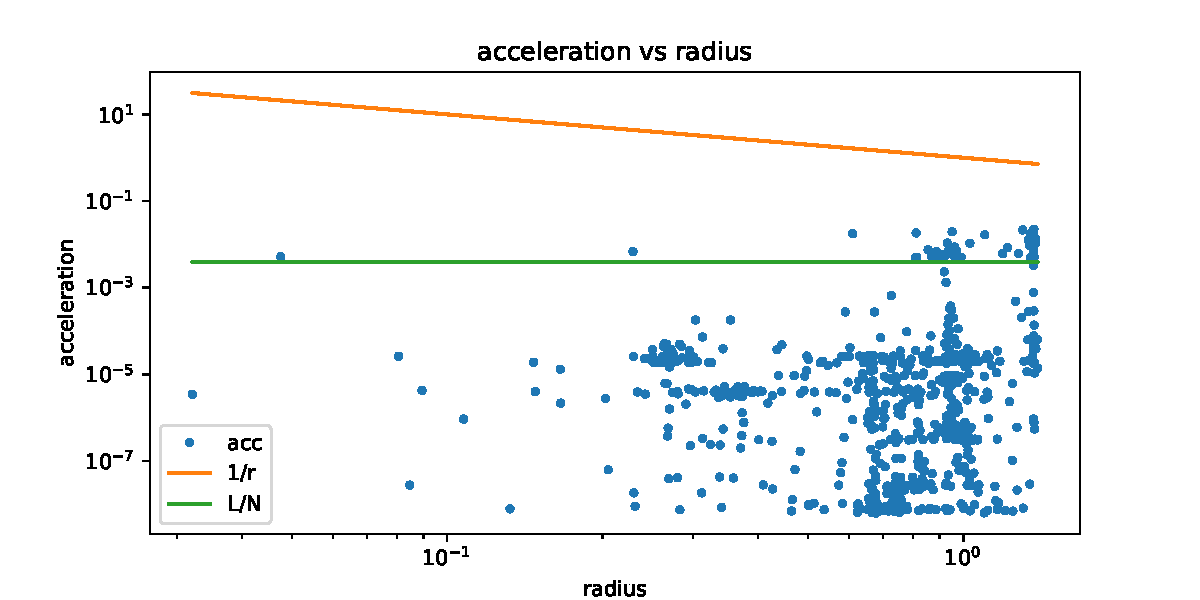
\includegraphics[width=\textwidth]{../figures/acc2.pdf}
        \end{figure} \ \\ 
        This is not what we expected.
